\scanpage{81}

\(I'_{f'}\quad (f_{i'}:\mathcal E_{i'}\longrightarrow
\mathcal E_{i=\tau(i')},\ \text{the }\alpha_{i'}\in\mathcal E)\)
are the same as in the case considered previously.

\uline{N.B.} This means in fact that we begin \unsure{to} ``plug the holes'' \deleted{of}
(of \(X'\)) corresponding to the \(i'\in I'\setminus I'_{f'}\), by replacing
\(\mathcal E'\) by the \deleted{\unsure{sub-}}quotient group of \(\mathcal E'\)
by the invariant subgroup generated by the
\(L_{i'}=\kappa_{i'}(T(\overline K))\)
\((i'\in I'\setminus I'_{f'})\), and \deleted{the} \unsure{\(\mathcal E_{i'}\)}
\((i'\in I'_{f'})\) by their images in the said quotient group, and forgetting
\deleted{the} \(I'\setminus I'_{f'}\), i.e. replacing \(I'\) by \(I'_{f'}\).

[To do things properly, we would have to express these operations also at the level of diagrams
of groupoids
\diagram{\begin{tikzcd}[ampersand replacement=\&]
\Pi'_{\unsure{D^*}} \arrow[r,dash] \& \Pi'_U \arrow[r] \& \unsure{\Pi'_e|\Pi_e}
\end{tikzcd}}
\(\ldots\)].

\margin{\deleted{\illegible{2} we would still have to \unsure{spell out}
\illegible{2} \unsure{some|the} points of \illegible{1}}}

This means then that in fact, we have brought ourselves back to the situation considered at the beginning,
where \(S'=\widehat f^{-1}(S)\)\ldots\ So in the end
the difference between the two points of view is not enormous, and
\deleted{\illegible{1}}\inserted{the one} adopted at the beginning has the advantage of
greater simplicity (everything is relative!)

\margin{80}

\scanpage{82}
\mspage{39}

11. Conditions on the systems of \deleted{\unsure{diagrams}}\inserted{groupoids}
obtained from geometric situations.

We have already mentioned some in passing, for example that the kernel groups of
\(\Pi_{D^*}-\Pi_e\) are abelian (with the Kummer isomorphism \(\kappa\))
and that the images are open subgroups, and the \(=\) for
the image of the \deleted{\illegible{1}} \(\pi_1\) in \(\Pi_U-\Pi_e\).
We are going to spell out again \inserted{and make precise} this in the framework of the interpretation
in terms of
\diagram{\begin{tikzcd}[ampersand replacement=\&]
T(\overline K) \arrow[r,"\kappa_i"] \& \mathcal E_i \arrow[r,hook,"\rho_i"] \&
\mathcal E \arrow[r,"p"] \& \Gamma
\end{tikzcd}}
(the ``dimension 1'' case --- we do not exclude the case \(I=\varnothing\) ---
the ``dimension 0'' case being trivial\ldots)

a) The image \inserted{\(\Sigma\)} of \(p\) is open, more precisely exists
open subgroup \(\Gamma'\subset\Gamma\) over which
\(\mathcal E\) has a section [and even an ``admissible section'' in a sense to be
defined later --- so as to exclude the ``trivial'' sections coming
from the \(\mathcal E_i\)\ldots].

b) The image \(\Sigma_i\) of \(\mathcal E_i\) in \(\Gamma\) is open, and
the extension \(\mathcal E_i\) of \(\Sigma_i\) by \(L_i\)
\((\simeq T(\overline K))\) is trivial. [In fact, we have a
\inserted{\uline{privileged}} class of splittings, called ``algebraic'', forming a
torsor under
\(K_i^*\,\unsure{\hookrightarrow}\,\varprojlim\unsure{(K_i^{*n})_n|(K_i^{*})_n}\),
cf. number 9 \unsure{]|?} --- but

\margin{81}

\scanpage{83}

we are not going to consider \inserted{for the moment} this additional piece of
structure\ldots)

\deleted{c) We must}

The rest of the \deleted{hypotheses}\inserted{conditions} essentially concerns
the structure of the groups \(\pi=\operatorname{Ker}(p:\mathcal E\to\Gamma)\) with
its \inserted{conjugacy classes of} \uline{subgroups}
\unsure{(or rather} the outer homomorphisms
\(\kappa_i:\deleted{\unsure{\widehat{\mathbb Z}(1)}}T\ (=T(\unsure{\overline K^*}))\longrightarrow\pi\),
and the way \(\Sigma\) operates by outer automorphisms on \(\pi\).
These conditions are expressed in a particularly simple way when the
\(\Sigma_i\subset\Gamma\) are \(=\Gamma\)
(``the points of \(S\) \inserted{\unsure{all}} rational over \(K\)'') i.e.
\(\mathcal E_i\to\Gamma\) surjective, a fortiori \(\Sigma=\Gamma\) i.e.
\(\mathcal E\to\Gamma\) surjective. We are going to restrict ourselves to this case. The general case follows
by a finite extension of the base field
[\unsure{over which} \deleted{we the}\inserted{each} points of
\(S\) not rational over \(K\)
\inserted{i.e. each \(\Sigma_i\ne\Gamma\)}
\deleted{\unsure{split up}\illegible{1}}\inserted{\unsure{gives|give} rise}
to \(n_i\) points, \deleted{\unsure{equal}}
\(n_i=[\Gamma:\Sigma_i]\) \unsure{\(\}\)} --- and \(X_{K'}\)
\deleted{\illegible{1}} \unsure{split|splits} into \(n=(\Gamma:\Sigma)\) connected components
which are geometrically connected] --- but I am too lazy to spell out as I should,
in the context of groupoids or of \deleted{\unsure{extensions}} homomorphisms of profinite
groups, the operation of extension of base fields\ldots\ It is understood that

\margin{82}

\scanpage{84}
\mspage{40}

the conditions I am going to describe will be invariant under extension \unsure{of the|of the} base field.

\deleted{c) There exists \(\unsure{\xi|\zeta}\in T\)
\((=\unsure{T(\overline K^*)})\) and conjugates}

c) \(\forall i\)\deleted{\illegible{1}}, the outer homomorphism
\[
\kappa_i:T\longrightarrow\pi
\]
is compatible with the outer action of \(\Gamma\) (operating on \(T\) by the
cyclotomic character \(\chi\), and on \(\pi\) thanks to the extension \(\mathcal E\)
of \(\Gamma\) by \(\pi\)). In other words, for \(\forall g\in\mathcal E\),
exists an \uline{\(\alpha\in\pi\)} (\uline{N.B.} not just
\(\alpha\in\mathcal E\)!) such that we have,
\[
\operatorname{int}(g)\kappa_i(\unsure{\xi|\zeta})
=\operatorname{int}(\alpha)\kappa_i(\chi(p(g))\unsure{\xi|\zeta})
\]
i.e.
\[
\operatorname{int}(\alpha^{-1}g)\kappa_i(\unsure{\xi|\zeta})
=\kappa_i(\chi(p(g))\unsure{\xi|\zeta})
\]
This means then that 1°) \(\alpha^{-1}g\) normalizes \(L_i=\kappa_i(T)\).
[and this means \(=\), probably, that \(\alpha^{-1}g\in\mathcal E_i\)
--- and that we can find such an \(\alpha\in\pi\)
\inserted{such that \(\alpha^{-1}g\in\mathcal E_i\)} comes from the hypothesis
\(\mathcal E_i\to\Gamma\) surjective --- we take a \(\beta\in\mathcal E_i\)
\inserted{\(\unsure{=}\alpha^{-1}g\)} having the \(=\) image as \(g\) in \(\Gamma\)
and we take \(\alpha=g\beta^{-1}\)] and that 2°) the \inserted{inner} action of
\(\beta=\alpha^{-1}g\) on \(T\) is nothing other than by multiplication
by \(\chi(g)=\chi(\beta)\) --- which (for \(\beta\in\mathcal E_i\)) is nothing other than the

\margin{83}

\scanpage{85}

condition already spelled out that the group homomorphism \(\kappa_i:T\to\mathcal E_i\)
is compatible with the action of \(\mathcal E_i\), operating on \(T\) via
\(\chi\circ p\mid\mathcal E_i\), and on itself by inner automorphisms.

So condition c) is not really new --- I spell it out again in
slightly different terms, because of its importance. It implies that the operation
\margin{\figure{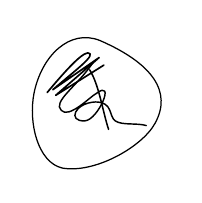
\begin{tikzpicture}[x=.012cm,y=-.012cm,line cap=round,line join=round]
\draw[line width=.45pt] (105,61) .. controls (73,48) and (43,77) .. (35,117)
 .. controls (29,148) and (39,190) .. (65,196)
 .. controls (99,202) and (149,174) .. (163,149)
 .. controls (182,115) and (160,85) .. (105,61);
\draw[line width=.52pt] (97,85) .. controls (81,109) and (54,126) .. (64,135)
 .. controls (72,144) and (95,120) .. (101,117)
 .. controls (122,101) and (103,145) .. (89,146)
 .. controls (70,147) and (78,127) .. (100,126)
 .. controls (119,126) and (114,141) .. (121,146)
 .. controls (128,151) and (144,148) .. (154,151);
\draw[line width=.55pt] (94,92) .. controls (104,108) and (108,137) .. (114,155);
\draw[line width=.60pt] (49,116) .. controls (65,97) and (84,75) .. (92,74)
 .. controls (103,75) and (78,93) .. (55,113)
 -- (104,79) -- (58,119) -- (109,87);
\end{tikzpicture}}}
of \(\Gamma\) on \(\pi\) is \uline{very} nontrivial (since
\(\chi:\Gamma\to\widehat{\mathbb Z}^{*}\) has an open image!)
--- it \unsure{was} not \(=\) obvious a priori
\inserted{(without deep arithmetic reasons!)} --- in view of the structure
of \(\pi\) that we are going to give --- that there exist such operations of \(\Gamma\)
on a \(\pi\)!

This condition \unsure{will be} supplemented by a nontriviality condition in the style of Weil.

d) \(\exists\eta\in T^*\)\unsure{.} (a basis of \(T\)), and
\(\alpha_i\in\pi\) (in order to conjugate \(\kappa_i\) into
\(\kappa'_i=\operatorname{int}(\alpha_i)\circ\kappa_i\))
\unsure{finally} an integer \(g\geq0\) and elements
\(\unsure{x_i,y_i}\in\pi\) \((1\leq i\leq g)\), such that we have

\margin{84}

\scanpage{86}
\mspage{41}

1°) the \(\kappa'_i(\eta)\), \deleted{\illegible{1}} and the
\(\unsure{x_i,y_i|x_j,y_j}\) generate the profinite group \(\pi\)

2°) They satisfy the relation
\[
\boxed{[x_1,y_1].[x_2,y_2]\ldots[x_g,y_g]\,
\kappa'_1(\eta)\kappa'_2(\eta)\ldots\kappa'_{\unsure{\nu|n}}(\eta)=1}
\]

3°) This relation, with the generators considered describes \(\pi\)
\inserted{(as a profinite group)} by generators and relations\ldots

\uline{N.B.} We know that under these conditions, \(g\) is uniquely determined,
for example by the fact that
\(\pi_{ab}/\deleted{\text{images of the}}\sum\kappa_i(T)\)
is a free \(\widehat{\mathbb Z}\)-module of rank \(2g\) --- \(\pi_{ab}\)
being free of rank \(2g+\nu-1\) where \(\nu=\operatorname{card}(I)\).

For the choice of \(\eta\), we know that if \(\eta\) works, then
\(\forall\ \chi(\alpha)\eta\) too (where \(\alpha\in\Gamma\)) --- up to taking
conjugates. So the \(\eta\) that work \deleted{form} contain
a subtorsor\inserted{of \(T^*\)} (under the open subgroup
\(\chi(\Gamma)\) of \(\widehat{\mathbb Z}^{*}\).

\deleted{Suppose for simplicity that \(g=0\):
We see then that if the system of the \(\kappa'_i(\eta)\) is a privileged system of generators
(in the sense of d) above) then the
\(\operatorname{int}(g)\kappa'_i(\eta)\) too for \(\forall g\in\mathcal E\),
[\unsure{\(=\)} \(\operatorname{int}(\alpha)\kappa'_i(\chi(g)\eta)\)
for suitable \(\alpha\in\pi\)]}

\margin{85}

\scanpage{87}
\mspage{42}

\margin{(\unsure{therefore|in} \(\chi:\Gamma\to\widehat{\mathbb Z}^{*}\) \unsure{epimorphism})}

\deleted{hence also the \(\kappa'_i(\chi(g)\eta)\). \unsure{Taking}
\(K=\mathbb Q\), we thus find by arithmetic means:

\uline{Proposition} Let \(\pi\) be the free \unsure{\(P\)}-group
\inserted{on \unsure{\(\nu-1\)|\(\nu\) generators}} \unsure{(}\uline{generated} by generators
\(\ell_1,\ldots,\ell_\nu\) satisfying the defining relation
\(\prod\ell_i=1\). Then for every \(\alpha\in\widehat{\mathbb Z}^{*}\),
we still have \(\prod\ell_i^\alpha=1\), and the \(\ell'_i=\ell_i^\alpha\)
with this relation describe the profinite group \(\pi\).}
In fact, since the structure of the group \(\pi\) is independent of \(K\),
taking \(K=\mathbb Q\) (and admitting that there exists a smooth projective
geometrically connected curve of genus \(g\) over \(\mathbb Q\), having \(\nu\) rational points over \(\mathbb Q\)!),
we find that if the \(\ell_i\), \deleted{\(\unsure{x_j,y_j}\)}
\((1\leq i\leq\nu\deleted{,\ \unsure{1\leq j\leq g}})\)
\deleted{work, then the} fit into a privileged system of generators
(with some \(\unsure{x_\alpha,y_\alpha}\)) then for
\(\forall\rho\in\widehat{\mathbb Z}^{*}\), we can find conjugates
\(\ell'_i\) of the \(\ell_i^\rho\) which fit in the \(=\) way.
Even for \(\rho=-1\) this is not entirely trivial\ldots

\deleted{\illegible{2}} Finally, \unsure{we are going to} state a draconian condition
of nontriviality of the operation of \(\Gamma\) on \(\pi\).
Let \(\mathcal E'\) be a subgroup \inserted{\uline{open} (hence}
of finite index) of \(\mathcal E\),
\inserted{\(\pi'=\pi\cap\mathcal E'=\operatorname{Ker}(\mathcal E'\to\Gamma')\)}
\deleted{\illegible{1} its image in \unsure{\(\mathcal E\)|\(\Gamma\)}
(which is open in \(\Sigma\)) so that}

\margin{86}

\scanpage{88}

\(\Gamma'\) the image of \(\mathcal E'\) in \(\Gamma\). We thus get an
extension of \(\Gamma'\) \((=\operatorname{Gal}(\overline K'/K'))\) over \(\pi'\),
hence also by \(\unsure{(\pi'_{ab})_{(\ell)}}\)
(\(\ell\) being a prime number), which is (we know this by d)) a
free \(\mathbb Z_\ell\)-module of finite type,
\inserted{on which \(\Gamma'\) operates}

[With a little work, we should be able to put on
\(\mathcal E'\to\Gamma\) a ``loop structure'' i.e. some
\(\mathcal E'_{i'}\), as for \(\mathcal E\), and describe in
\(\unsure{(\pi'_{ab})_{(\ell)}}\)
\inserted{the sum} of the images of the \deleted{\illegible{1}} \(L'_{i'}\),
on which \(\Gamma'\) operates \inserted{therefore} via the character \(\chi\).

\margin{This is done very elegantly in the setting
\diagram{\begin{tikzcd}[ampersand replacement=\&]
\Pi_{D^*} \arrow[r] \& \Pi_U \arrow[r] \& \Pi_e
\end{tikzcd}}}

We are interested in the quotient of \(\unsure{(\pi'_{ab})_{(\ell)}}\) by
\unsure{this submodule|these submodules} which is relatively trivial (the ``abelian variety'' part of the
\(\ell\)-adic module under consideration). This being said

\textcircled{e} we require that the representation of \(\Gamma'\) on this be
``pure of weight 1'' --- \deleted{\unsure{i.e.} we have} and that the characteristic polynomials
of the Frobenius elements (which have coefficients \(\in\mathbb Z\), not just
\(\in\mathbb Z_\ell\)) be \uuline{independent} of \(\ell\).

\margin{\figure{\begin{tikzpicture}[x=1cm,y=1cm,line cap=round]
\draw[line width=.34pt] (.04,.30) .. controls (-.30,.35) and (-.42,.13) .. (-.40,-.08)
 .. controls (-.39,-.36) and (-.14,-.39) .. (.08,-.23)
 .. controls (.36,-.01) and (.28,.27) .. (.04,.30);
\node[inner sep=0pt] at (-.08,-.02) {$e$};
\draw[line width=.29pt] (-.06,-.71) .. controls (.01,-1.68) and (-.08,-2.52) .. (.02,-3.52)
 .. controls (.09,-4.37) and (.08,-5.24) .. (.15,-5.98)
 -- (.07,-6.30);
\end{tikzpicture}}}
\margin{87}

\scanpage{89}
\mspage{43}

\Needspace{4\baselineskip}
12. \uline{The topological analogy}\par\nobreak
Let \(X\) be a compact
orientable (topological) \deleted{manifold}\inserted{surface}, \(S\) a finite subset of \(X\). If \(X\) is connected, we consider
the set \inserted{\unsure{\(\omega\)}} \unsure{of the|its} two orientations,
we use it to twist the group \(\mathbb Z\), whence a group \unsure{\(T\)}
\[
T=\mathbb Z\mathop{\wedge}\limits_{\pm1}\unsure{\{\omega\}|\omega}.
\]
isomorphic (noncanonically) to \(\mathbb Z\). More generally, suppose
given such a group \(T\),
\inserted{i.e. an \(\omega\in\unsure{\operatorname{Ob}}\mathrm{Ens}_2\)}
--- a \(T\)-orientation of \(X\) will by definition be an \unsure{element}
of the set \(\operatorname{Or}(X)\mathop{\wedge}\limits_{\{\pm1\}}\omega\).

[in the preceding case, \(X\) will thus be canonically \(T\)-oriented\ldots]

Let us consider the fundamental groupoid of \(X\setminus S=U\), say \(\Pi_U\),
and the fundamental groupoid \inserted{\(\Pi_{D^*}\)} of germs
of spaces of \(X\) around \(S\), \uline{deprived} of \(S\)
\inserted{\deleted{\unsure{of the}} groupoids \unsure{?}}
(of germs of universal coverings of \(X\setminus S\) in a neighborhood of \(S\)).
We thus have a canonical functor
\diagram{\begin{tikzcd}[ampersand replacement=\&]
\unsure{\Pi_{D^*}} \arrow[r,dash] \& \Pi_U
\end{tikzcd}}
and on the other hand, \deleted{\illegible{2}} if \(X\) is \(T\)-oriented, we have an
additional structure

\margin{88}

\scanpage{90}

of interest on \inserted{the groupoid} \(\Pi_{D^*}\): the local system of
its \(\pi_1\) is canonically isomorphic to \(T\).

Associating to every \(X\) which is \(T\)-oriented the system
\[
\Pi_{D^*}\longrightarrow\Pi_{\unsure{X|U}},\qquad
\kappa:T_{(\Pi_{D^*})}\simeq\pi_1(\Pi_{D^*}/e),
\]
we find a 2-equivalence between the topological 2 category of
\deleted{\unsure{manifolds}} pairs \((X,S)\) of a
\inserted{(for homeomorphisms up to isotopy\ldots)}
\unsure{compact \(T\)-oriented manifold}, and of the 2-category of the preceding
systems \inserted{(for equivalences)}, \unsure{(}which satisfy the conditions

a) \(\pi_0(\Pi_{D^*})\), \deleted{\unsure{and}} \(\pi_0(\Pi_X)\) finite

b) For \unsure{every|\(\forall\)} connected component of \(\Pi_U\), say
\(\Pi_{U_0}\), and the part \(\unsure{\Pi_{D_0^*}}\) above it, spelling out the
\unsure{groupoid} situation by \unsure{a|a}
\inserted{group \(\pi\) and a} family of homomorphisms
\(T\xrightarrow{\kappa_i}\pi\), we have (\uline{N.B.} the whole thing \unsure{depends|depending} on choices,
but \(\pi\) is intrinsic as an outer group, and the \(\kappa_i\)
\unsure{as homomorphisms} that are outer --- \unsure{define|defining} a ``\(T\)-loop structure
on \(\unsure{S}\) ---) we have the following.

\margin{89}
